%*----------- SLIDE -------------------------------------------------------------
\begin{frame}[t]{O problema da localização} 
    \transdissolve[duration=0.5]
    Quando um robô móvel se move pelo meio ele pode sofrer problemas por não ter como usar sinais de GPS.
    %\newline
        \begin{columns}[t]
            \column{.05\linewidth}
            \column{.4\linewidth}
            \begin{figure}
                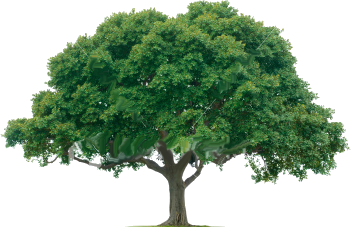
\includegraphics[width=1\textwidth]{arvore.png}
                \caption{Arvore \cite{arvore:online}}
            \end{figure}
            \column{.6\linewidth}
            \begin{figure}
                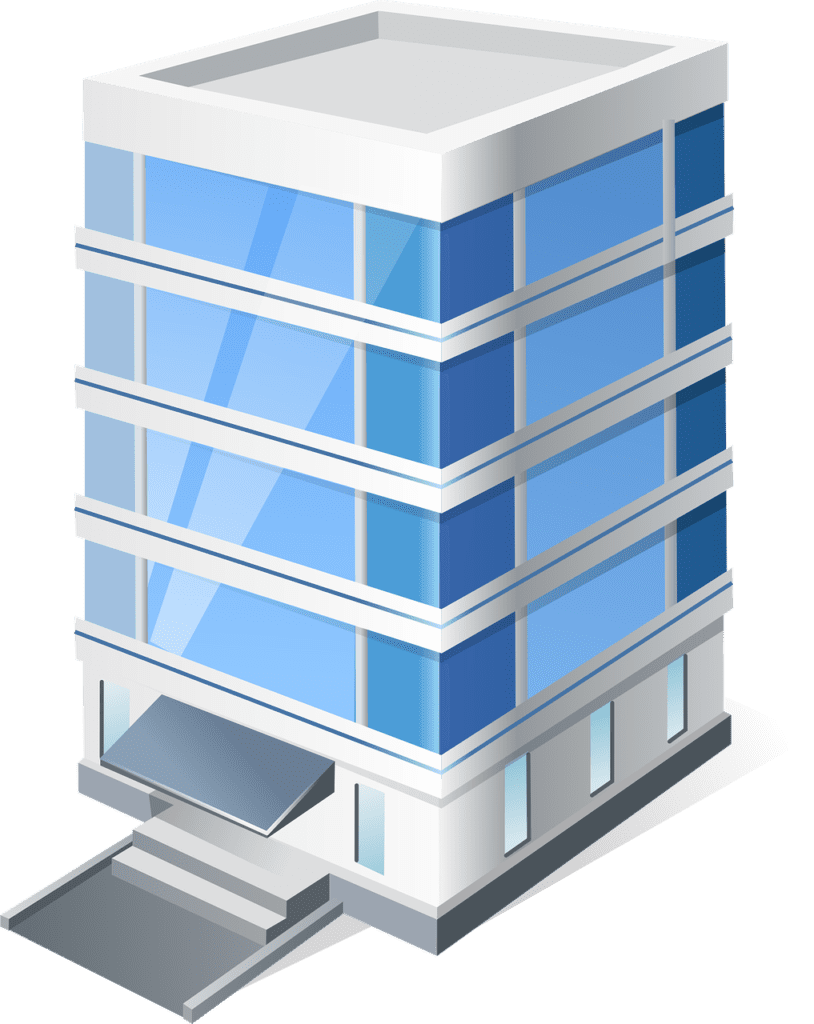
\includegraphics[width=0.3\textwidth]{predio.png}
                \caption{Prédio \cite{predio}}
            \end{figure}

        \end{columns}
\end{frame}

%*----------- SLIDE -------------------------------------------------------------
\begin{frame}[t]{Para solucionar} 
    \transdissolve[duration=0.5]
    \begin{center}
        \begin{figure}
            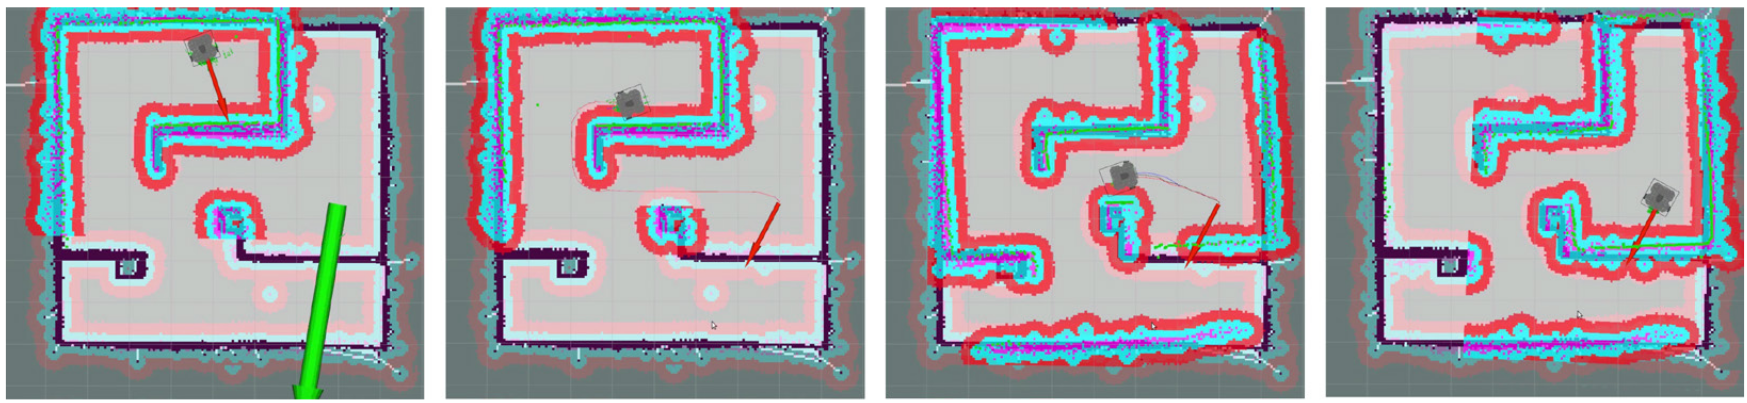
\includegraphics[width=1\textwidth]{2d_nav_goal.png}
            \caption{Mapeamento \cite{Turtlebot}}
        \end{figure}
    \end{center}

\end{frame}


%*----------- SLIDE -------------------------------------------------------------
\begin{frame}[t]{Dois tipos principais de mapeamento} 
    \transdissolve[duration=0.5]
    Para mapear um ambiente são utilizados principalmente dois tipos de mapas.
    \begin{columns}[t]
        \column{.03\linewidth}
        \column{.42\linewidth}
        \begin{figure}
            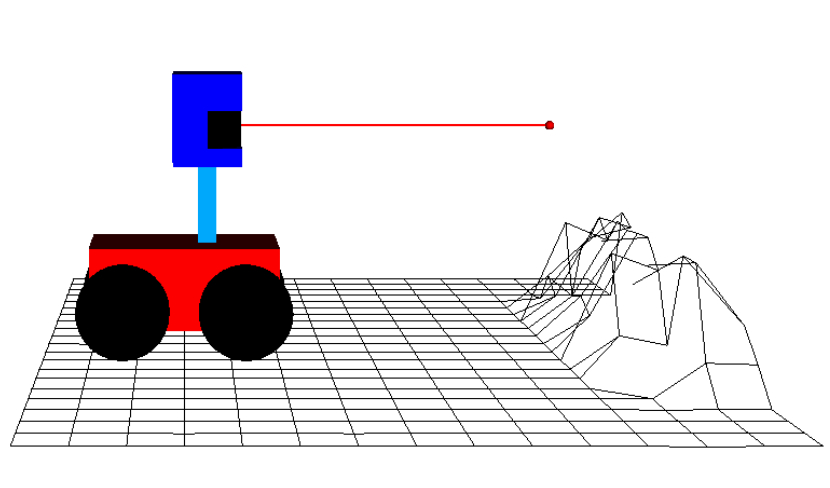
\includegraphics[width=1\textwidth]{elevation_map2.jpg}
            \caption{Elevation maps \cite{article}}
        \end{figure}
        \column{.6\linewidth}
        \begin{figure}
            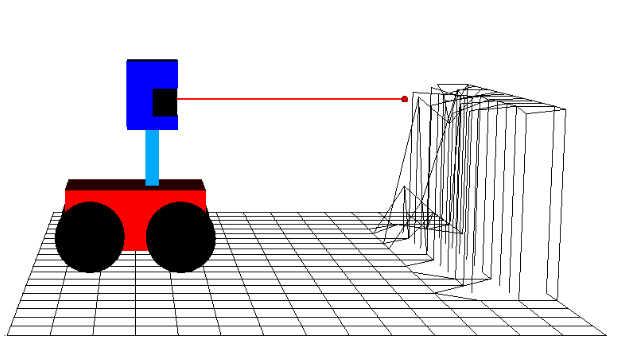
\includegraphics[width=.73\textwidth]{mls.jpg}
            \caption{Multi-level surface \cite{article}}
        \end{figure}
    \end{columns}

\end{frame}
%-

%*----------- SLIDE -------------------------------------------------------------
\begin{frame}[t]{\textit{Elevation maps}} 
    \transdissolve[duration=0.5]    
    %\newline
        \begin{columns}[t]
            \column{.05\linewidth}
            \column{.4\linewidth}
                \begin{enumerate}
                    \item Oferece um fraco suporte para a localização do robô.
                    \item Mapeia apenas as superficies horizontal.
                    \item Estruturas verticais não podem ser usadas para localização.
                \end{enumerate}
            \column{.6\linewidth}
            \begin{center}
            %\centerline{
                \begin{figure}
                    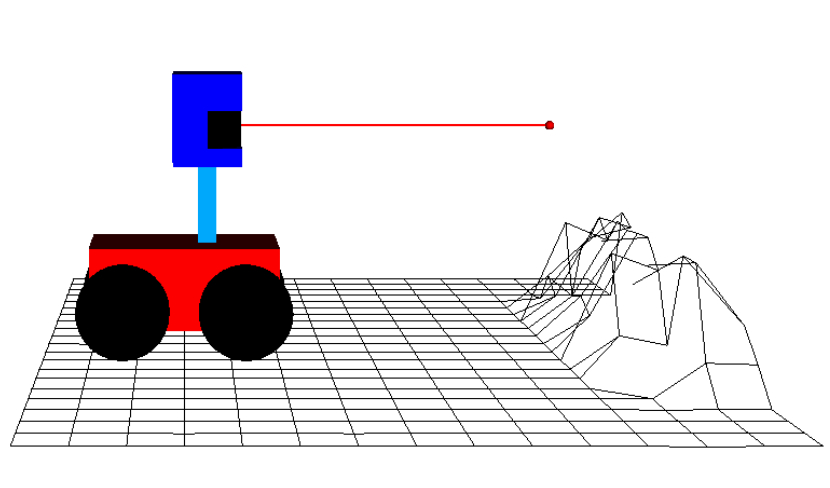
\includegraphics[width=1\textwidth]{elevation_map2.jpg}
                    \caption{Elevation maps \cite{article}}
                \end{figure}
            %}
            \end{center}
        \end{columns}
%*----------- notes
    \note[item]{Notes can help you to remember important information. Turn on the notes option.}
\end{frame}

%*----------- SLIDE -------------------------------------------------------------
\begin{frame}[t]{\textit{Multi-Level Surface maps}} 
    \transdissolve[duration=0.5]
    %\newline
        \begin{columns}[t]
            \column{.05\linewidth}
            \column{.4\linewidth}
                \begin{enumerate}
                    \item Ser uma extensão do \textit{elevation map}.
                    \item Representam intervalos que correspondem aos objetos verticais.
                    \item Podem representar diversos níveis.
                \end{enumerate}
            \column{.6\linewidth}
            \begin{center}
            %\centerline{
                \begin{figure}
                    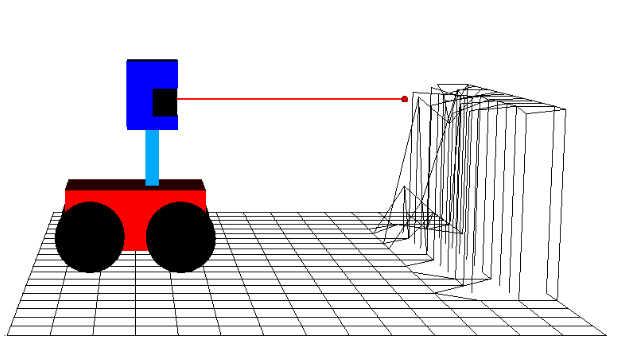
\includegraphics[width=1\textwidth]{mls.jpg}
                    \caption{Multi-level surface \cite{article}}
                    % \roundpic[xshift=0cm,yshift=0cm]{2.5cm}{6cm}{pista}
                    %\caption{Pista de corrida \cite{agostini2007}}
                \end{figure}
            %}
            \end{center}
        \end{columns}
%*----------- notes
    \note[item]{Notes can help you to remember important information. Turn on the notes option.}
\end{frame}

%-
%*----------- SLIDE -------------------------------------------------------------
% \begin{frame}[c]{Objetivo} 
%     \transdissolve[duration=0.5]
   
%     \begin{center}
%         \Wider{
%         \begin{shaded}
%         \begin{center}
%             \vspace*{0.5cm}
%             \resizebox{!}{0.35cm}{
%                 \color{bg} Usar o \textit{multi-level surface map} para localização em ambientes externos.
%             }
%         \end{center}
%         \end{shaded}
%         }
%     \end{center}
    
% \end{frame}

